\documentclass[11pt, a4paper]{report}
\usepackage[utf8]{inputenc}%codification of the document
\usepackage[french]{babel}
\usepackage{geometry}
\usepackage{times}
\usepackage{graphicx}
\usepackage{multicol}
\usepackage{float}
\usepackage{subcaption}
\usepackage{comment}
\usepackage{hyperref}
\usepackage{listings}
\usepackage{color}
\usepackage[dvipsnames]{xcolor}
\definecolor{EnoncerQuestions}{RGB}{10, 84, 68}
\definecolor{EnincerExercice}{RGB}{158, 19, 24}

\definecolor{lightgray}{rgb}{.98,.98,.98}
\definecolor{darkgray}{rgb}{.4,.4,.4}
\definecolor{blue}{rgb}{0.5, 0.2, 0.82}
\definecolor{purple}{rgb}{0.7, 0, 0.6}

\lstdefinelanguage{C}{
	keywords={typeof, new, true, false, catch, function, return, null, catch, switch, var, if, in, while, do, else, case, break},
	keywordstyle=\color{blue}\bfseries,
	ndkeywords={class, export, boolean, throw, implements, import, this},
	ndkeywordstyle=\color{darkgray}\bfseries,
	identifierstyle=\color{black},
	sensitive=false,
	comment=[l]{//},
	morecomment=[s]{/*}{*/},
	commentstyle=\color{blue}\ttfamily,
	stringstyle=\color{purple}\ttfamily,
	morestring=[b]',
	morestring=[b]"
}

\lstset{
	language=C,
	backgroundcolor=\color{lightgray},
	extendedchars=true,
	basicstyle=\footnotesize\ttfamily,
	showstringspaces=false,
	showspaces=false,
	numbers=left,
	numberstyle=\footnotesize,
	numbersep=9pt,
	tabsize=2,
	breaklines=true,
	showtabs=false,
	captionpos=b
}
\author{Badmavasan KIROUCHENASSAMY \& Caroline SCHMID}
\date{}
\title{Projet tutoré de Structures de Données - Graphes et Combinatoires : Problème du flot maximum}
\begin{document}
	\pagenumbering{roman}
	\begin{titlepage}
		\begin{center}
			
			\vspace*{1cm}
			
			\begin{figure}[h]
				\centering
				
\includegraphics[width=0.4\textwidth]{images/LOGO_Polytech-lille.jpg}
				\hspace{2cm}
				
\includegraphics[width=0.4\textwidth]{images/logo_ulille_transparent.png}
			\end{figure}
			
			\vspace*{2cm}
			
			\rule{1\textwidth}{.8pt}
			
			\LARGE{\textsc{Projet Informatique \& Statistique\\-\\Anti-monopoly}}
			
			\vspace*{1cm}
			
			\LARGE{\textsc{Conception}}
			\vspace*{1cm}
			
			\small{IS2A3 - Mardi 1er juin 2021}
			
			\vspace*{0.5cm}
			\rule{1\textwidth}{.10pt}
		
			\vspace*{2.352cm}
			
			\large{\textit{Encadrants :} Santiago BRAGAGNOLO\\Pablo TESONE}
			
			\vspace*{0.1cm}	        
			
			\large{\textit{Auteurs :} {Caroline SCHMID\\Brinda TSOBGNI}}
			
			
			
			
		\end{center}
		
	\end{titlepage}
	
	
	%\setcounter{tocdepth}{2}
	\tableofcontents
	
	
	\chapter{Contexte du projet}
	\pagenumbering{arabic}
	
	Au cours de ce projet, on représente une partie de Monopoly dont la simulation est basée sur des joueurs pouvant être soit Prudents, soit Agressifs. L'un des joueur est l'État, il ne prend pas directement part au jeu mais en est un élément important.
	
	De plus, la construction du jeu dépend de la configuration que l'utilisateur choisit en lançant le programme. Ce choix détermine les valeurs des cases comme par exemple la valeur de la taxe à payer, mais également les moyens fournis aux différents joueurs en lançant le jeu, car dans certaines configurations les joueurs ne partent pas d'un même montant.
	
	Le plateau est constitué de cases de différents types, ces derniers déterminant les actions à réaliser en arrivant sur la case.
	
	Les joueurs sont caractérisés par leur style de jeu.
	
	La simulation crée les différentes entités nécessaires (un plateau, des joueurs, ...) et les fait jouer jusqu'à ce que soit l'État n'a plus de moyens, soit qu'il ne reste plus qu'un seul joueur ou encore que l'utilisateur décide de mettre fin à la partie.
	
	
	
	\chapter{Détail de la Simulation}
	
	La simulation peut être découpée en 3 étapes :
	
	\begin{enumerate}
		
		\item Initialisation du jeu
		
		\item Déroulement du jeu
		
		\item Résultats
	
	\end{enumerate}
	
	
	\section{Initialisation du jeu}
	
	On demande à l'utilisateur d'indiquer :
	
	\begin{enumerate}
		
		\item la configuration dans laquelle il veut lancer la simulation
		
		\item le nombre de joueurs pour chaque style de jeu
		
	\end{enumerate}
	
	Le plateau ainsi que la liste des joueurs sont créés en fonction des informations indiquées. L'État est également ajouté à la liste des joueurs mais est traîté de manière différente des autre joueurs.
	
	\section{Déroulement du jeu}

	Le jeu se déroule de la manière suivante : chaque joueur joue à tour de rôle jusqu'à ce que la fin de la partie soit déclarée. Pour chaque joueur, sauf l'État, le dé est lancé, donnant un résultat de 1 à 6. le joueur qui a la main avance d'autant de cases et réalise l'action indiquée dessus. Les actions peuvent être les suivantes :

	\begin{itemize}
		
		\item Si la case est un investissement et si l'investissement n'est pas encore la propriété d'un joueur, s'il appartient à l'État, le joueur peut décider de l'acheter ou pas, dépendant de son style de jeu et de ses moyens. Si l'investissement appartient déjà à un autre joueur, celui qui joue son tour doit payer au propriétaire un pourcentage de la valeur de l'investissement.
		
		\item Si la case est une loi antitrust et si les propriétés du joueur dépassent un seuil fixé par l'État, il doit revendre certaines de ses possessions à moitié prix à l'État pour se trouver en dessous de ce seuil. Le joueur, dépendant de son mode de jeu choisira les propriétés dont il veut se séparer.
		
		\item Si la case est un bureau des finances publiques, le joueur doit payer une taxe sur la somme d'argent qu'il a. La taxe est d'un certain pourcentage indiqué dans la case et est à payer à l'État.
		
		\item Si la case est une subvention, le joueur reçoit de l'État le montant indiqué dans la case.
		
		\item Si la case est une case de repos, le joueur ne fait rien.
		
	\end{itemize}
	Un joueur sort du jeu s'il n'a plus de moyen financier.\\
	Le jeu prend fin si l'une des conditions suivantes est remplie :
	
	\begin{enumerate}
		
		\item Il ne reste plus qu'un seul joueur sur le plateau
		
		\item L'État n'a plus de moyen financier, il a échoué
		
		\item L'utilisateur décide d'interrompre la partie.
		
	\end{enumerate}
	
	
	\section{Résultats}
	
	En premier est affiché la raison pour laquelle le jeu a été interrompu.
	
	Les résultats sont affichés par ordre : sont indiqués, le vainqueur, le montant de ses investissements, ses moyens financiers et son patrimoine ; puis vient le tour du second avec les mêmes informations et ainsi de suite.
	
	
	
	\chapter{Schéma UML des classes}
	
	\begin{figure}[h]
		\centering
		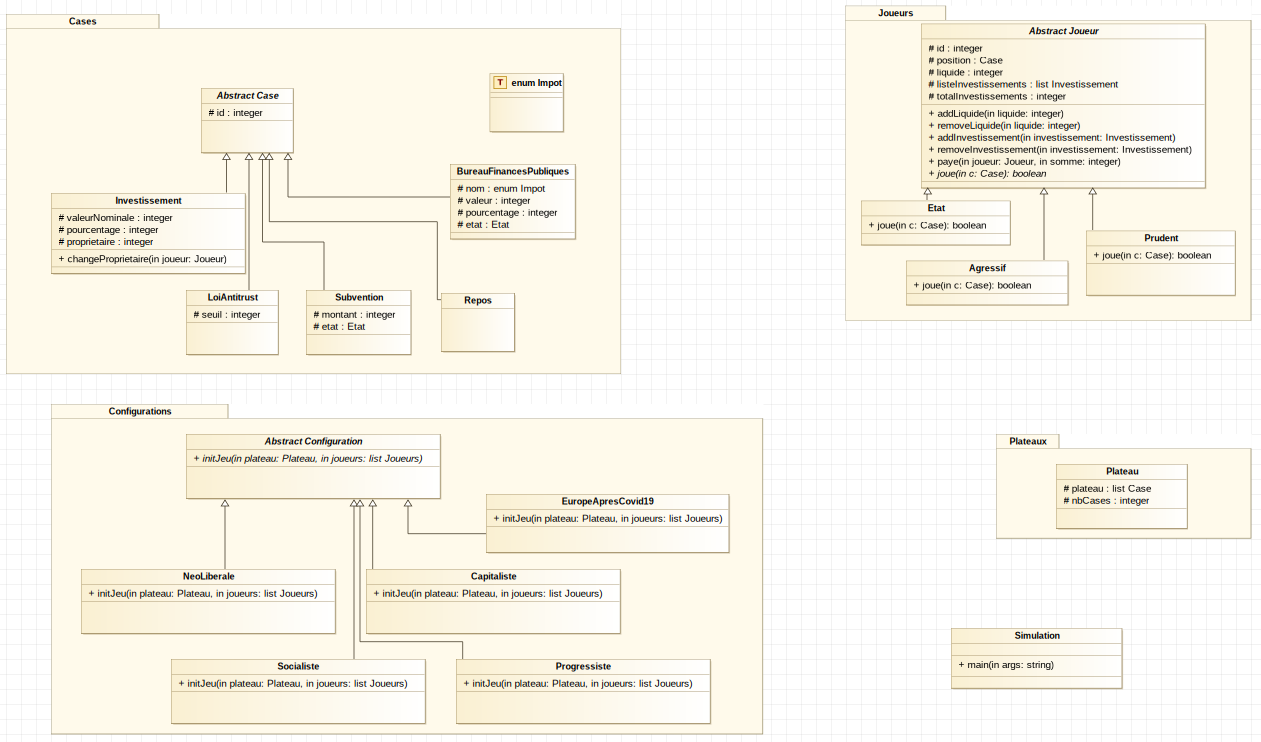
\includegraphics[width=1\textwidth]{images/UML2.png}
	\end{figure}
	
	Toute les classes sont regroupées dans un package \verb|Monopoly|.
	
	Le projet est découpé en 5 sous-structures :
	
	\begin{itemize}
		\pagebreak
		
		\item Le package \verb|Cases| contenant les différents types de cases, chacun représenté par une classe, toutes héritant de la classe \verb|Case|, classe abstraite permettant d'indiquer que tous ces types sont des cases.\\
		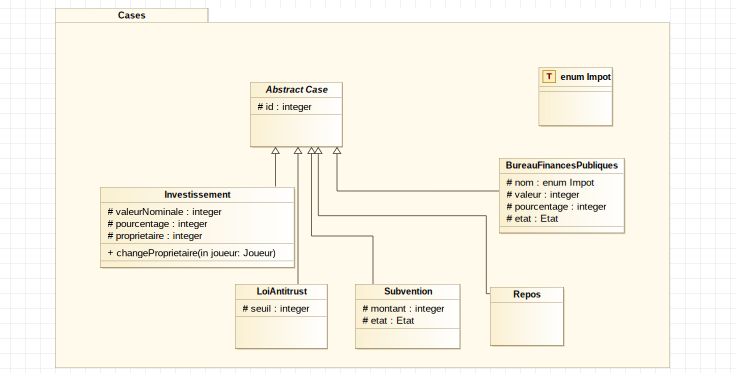
\includegraphics[width=1\textwidth]{images/Cases2.png}
		
		\item Le package \verb|Joueurs| contenant les différents styles de jeu, chacun représenté par une classe dont la classe \verb|Etat|, toutes héritant de la classe \verb|Joueur|, classe abstraite permettant d'indiquer que tous ces styles sont des joueurs.\\
		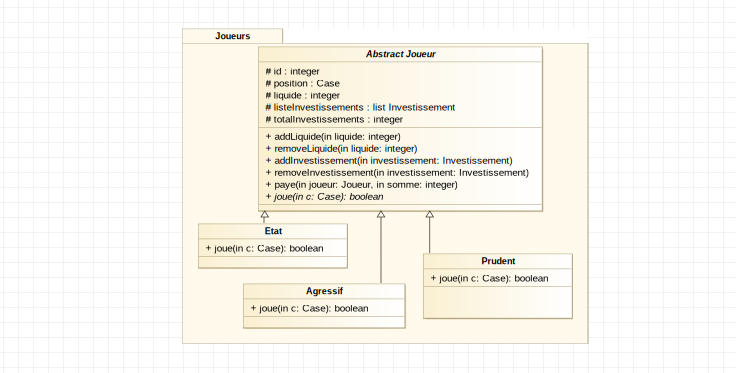
\includegraphics[width=1\textwidth]{images/Joueurs2.png}
		
		\pagebreak
		
		\item Le package \verb|Plateaux| contient pour le moment qu'une classe \verb|Plateau| permettant de construire le plateau et d'accéder à ses attributs. Une extension serait possible en ajoutant d'autres plateaux.\\
		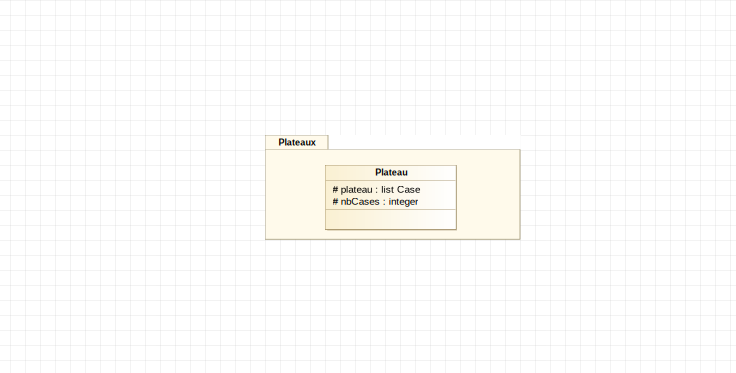
\includegraphics[width=1\textwidth]{images/Plateaux2.png}
		
		\item Le package \verb|Configurations| contenant les différents environnements dans lequels le jeu peut se dérouler, chacun représenté par une classe, toutes héritant de la classe \verb|Configuration|, classe abstraite permettant d'indiquer que tous ces types sont des configurations.\\
		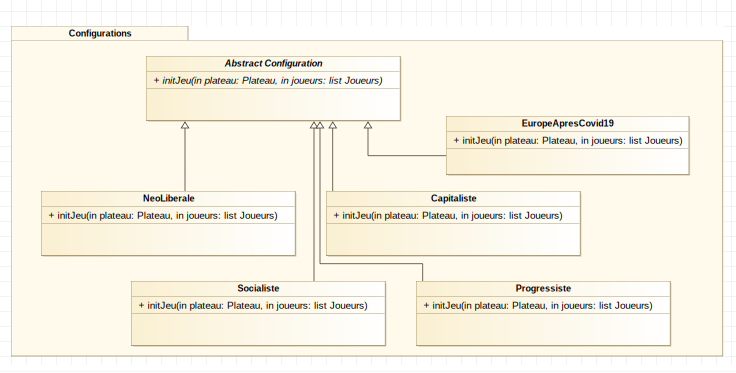
\includegraphics[width=1\textwidth]{images/Configurations2.png}
		
		\pagebreak
		
		\item La classe \verb|Simulation|, le main. Contient la création, le déroulement et la fin du jeu.\\
		\includegraphics[width=1\textwidth]{images/Simulation2.png}
		
	\end{itemize}
	
	
	\chapter{Choix des structures de données non-primitives}
	
	Deux structures non-primitives de la librairie $java.util$ ont été mises en œuvre : '$ArrayList$' et '$LinkedList$'.
	
	La '$ArrayList$' constitue le parcours. Elle contient les cases du plateau. On a choisi cette structure de données car les valeurs contenues ne changent pas dans le sens où on ne retire pas ou on n'ajoute pas de valeur au cours du jeu. Une fois la structure construite, aucun ajout ou suppression n'est réalisé.
	
	Une '$LinkedList$' contient les participants prenant part au jeu. Ce choix s'est fait car les joueurs perdant sont sortis de la liste, et le coût mémoire est moins important dans cette structure étant donné que c'est une liste chaînée.
	
	Une seconde structure '$LinkedList$' est utilisée par chaque joueur pour contenir les investissements de chacun. Les raisons de ce choix sont les mêmes qu'expliqué au dessus : les joueurs achètent et revendent leurs investissements tout au long du jeu, il faut donc les ajouter et les supprimer des listes. Les '$LinkedList$' sont les structures de données les plus efficaces pour les ajouts et suppressions.
	
	
	\chapter{Tests Unitaires}
	
	Un test unitaire peut être réalisé par constructeur et par nombre d'attributs dans la classe. On peut vérifier que la valeur affectée est bien celle stockée dans l'attribut. Ceci peut être intéressant si un attribut est initialisé autrement que par une affectation simple, en appelant une fonction, en opérant une boucle, en réalisant un calcul ou autre. Cette situation ne devrait pas apparaître dans ce projet, on ne le réalisera donc pas.
	
	La classe Simulation ne contenant qu'un main, dans l'état actuel des choses, elle ne sera pas testée.
	
	Les tests unitaires peuvent être réalisés par package.
	
	
	\section{Cases}
	
	Le package \verb|Cases| : la seule méthode prévue pour l'ensemble des classes de ce package est dans la classe \verb|Investissement|, \verb|changeProprietaire|. Vérification que le changement de propriétaire d'un investissement s'effectue correctement.
	
	
	
	\section{Joueurs}
	
	Le package \verb|Joueurs| : chaque méthode peut être testée. certaines nécessiteront plusieurs tests pour s'assurer que les différentes actions ont été réalisées correctement. Par exemple, la méthode \verb|paye| devra effectuer correctement la modification sur le montant financier du joueur payant la somme en question, mais également la modification correcte sur le montant financier de celui étant payé. De plus, la méthode \verb|joue| peut être testée pour vérifier que les valeurs attribuées sont bien les bonnes. On peut également mettre un joueur dans une situation et vérifier que son action est cohérente avec son style de jeu.
	
	
	
	\section{Plateaux}
	
	Le package \verb|Plateaux| : le plateau ne présente aucune méthode intéressante à tester étant donné qu'il sera construit dans un premier temps dans une classe de configuration.
	
	
	
	\section{Configurations}
	
	Le package \verb|Configurations| : chaque classe de ce package initialise la liste des joueurs et le plateau de jeu de manière différente. On peut tester que chaque action est réalisée correctement et qu'elle correspond à la configuration dans laquelle elle est. Par exemple, vérifier qu'un plateau de configuration Socialist ait bien fixé des taxes élevées. L'inverse serait contradictoire avec la configuration choisie par l'utilisateur.
	
	
	
\end{document}
